%\title{LaTeX Portrait Poster Template}
%%%%%%%%%%%%%%%%%%%%%%%%%%%%%%%%%%%%%%%%%
% a0poster Portrait Poster
% LaTeX Template
% Version 1.0 (22/06/13)
%
% The a0poster class was created by:
% Gerlinde Kettl and Matthias Weiser (tex@kettl.de)
% 
% Adapter by Jens Buysse for Hogeschool Gent
% This template has been downloaded from:
% http://www.LaTeXTemplates.com
%
% License:
% CC BY-NC-SA 3.0 (http://creativecommons.org/licenses/by-nc-sa/3.0/)
%
%%%%%%%%%%%%%%%%%%%%%%%%%%%%%%%%%%%%%%%%%

%----------------------------------------------------------------------------------------
%	PACKAGES AND OTHER DOCUMENT CONFIGURATIONS
%----------------------------------------------------------------------------------------

\documentclass[a0,portrait]{a0poster}

\usepackage{multicol} % This is so we can have multiple columns of text side-by-side
\columnsep=100pt % This is the amount of white space between the columns in the poster
\columnseprule=3pt % This is the thickness of the black line between the columns in the poster

\usepackage[svgnames]{xcolor} % Specify colors by their 'svgnames', for a full list of all colors available see here: http://www.latextemplates.com/svgnames-colors

\usepackage{times} % Use the times font
%\usepackage{palatino} % Uncomment to use the Palatino font

\usepackage{graphicx} % Required for including images
\graphicspath{{figures/}} % Location of the graphics files
\usepackage{booktabs} % Top and bottom rules for table
\usepackage[font=small,labelfont=bf]{caption} % Required for specifying captions to tables and figures
\usepackage{amsfonts, amsmath, amsthm, amssymb} % For math fonts, symbols and environments
\usepackage{wrapfig} % Allows wrapping text around tables and figures
\usepackage[export]{adjustbox}

\begin{document}

%----------------------------------------------------------------------------------------
%	POSTER HEADER 
%----------------------------------------------------------------------------------------

% The header is divided into two boxes:
% The first is 75% wide and houses the title, subtitle, names, university/organization and contact information
% The second is 25% wide and houses a logo for your university/organization or a photo of you
% The widths of these boxes can be easily edited to accommodate your content as you see fit

\begin{minipage}[t]{0.75\linewidth}
\VeryHuge \color{HoGentAccent1} \textbf{Analyse van nummerplaatdetectie aan de parking van UGent Campus Sterre en Campus Coupure.} \color{Black}\\ % Title
\Huge\textit{}\\[2.4cm] % Subtitle
\huge \textbf{Carly Angelo, Wannes Van Dorpe, Lotte Van Steenberghe}\\[0.5cm] % Author(s)
\huge Hogeschool Gent, Valentin Vaerwyckweg 1, 9000 Gent\\[0.4cm] % University/organization
\Large \texttt{angelo.carly.y7553@student.hogent.be} \\
\end{minipage}
%
\begin{minipage}[t]{0.25\linewidth}
\includegraphics[width=13cm,right]{figures/HOGENT_Logo_Pos_rgb.png} 

\end{minipage}

\vspace{1cm} % A bit of extra whitespace between the header and poster content

%----------------------------------------------------------------------------------------

\begin{multicols}{2} % This is how many columns your poster will be broken into, a portrait poster is generally split into 2 columns

%----------------------------------------------------------------------------------------
%	ABSTRACT
%----------------------------------------------------------------------------------------

\color{HoGentAccent1} % Navy color for the abstract

\begin{abstract}

In dit onderzoek werd nagegaan in welke mate het mogelijk is om nummerplaatdetectie uit te voeren op UGent Campus Sterre en Campus Coupure op een goedkope, milieuvriendelijke en gebruiksvriendelijke wijze dat voldoet aan de normen van de GDPR. Hiervoor werd gebruik gemaakt van een Raspberry Pi met de PiNoIR-Cam en het open-source framework OpenALPR. Uit het onderzoek bleek dat de voorgestelde implementatie van Vado Solutions wel degelijk mogelijk is onder de GDPR, alsook dat het voorgestelde systeem met de Raspberry Pi wel degelijk mogelijk is met een gemiddelde nauwkeurigheid van 95.4\%. Dit resultaat stelt de weg open naar breder onderzoek voor een volledige implementatie met deze technologieën.
\end{abstract}
%----------------------------------------------------------------------------------------
%	INTRODUCTION
%----------------------------------------------------------------------------------------

\color{HoGentAccent1} 
\section*{Introductie}
\color{black}
\color{black}
Dit onderzoek ging na in welke mate het mogelijk is nummerplaatdetectie op te stellen op de Campus Coupure en Campus Sterre van UGent. Hiervoor werd er bekeken in hoeverre de GDPR invloed heeft op nummerplaatdetectie. Daarnaast werden er maatregelen opgesteld om een nauwkeurige detectie te verkrijgen, waarop er vervolgens een testopstelling gemaakt werd om na te gaan of een dit wel degelijk mogelijk is op UGent.

Zo waren de volgende drie onderzoeksvragen bekomen:
\begin{itemize}
	\item Is nummerplaatdetectie een haalbare techniek omtrent GDPR?
	\item Welke maatregelen moeten er genomen worden om succesvol nummerplaatdetectie te implementeren?
	\item Kan men nummerplaatdetectie succesvol uitvoeren met een Raspberry Pi op de campus Coupure en Sterre van UGent?
\end{itemize}
%----------------------------------------------------------------------------------------
%	GEOLOGY
%----------------------------------------------------------------------------------------

\color{Black} % DarkSlateGray color for the rest of the content
\color{HoGentAccent1} 

\section*{Experimenten}
\color{black}

Om de nauwkeurigheid van de opstelling te testen werden er op de vier uitgangen foto's genomen van alle auto's. Vervolgens werd de nummerplaatdetectie hierop uitgevoerd m.b.v. OpenALPR en werden deze resultaten vergeleken.

\begin{center}
	\centering
	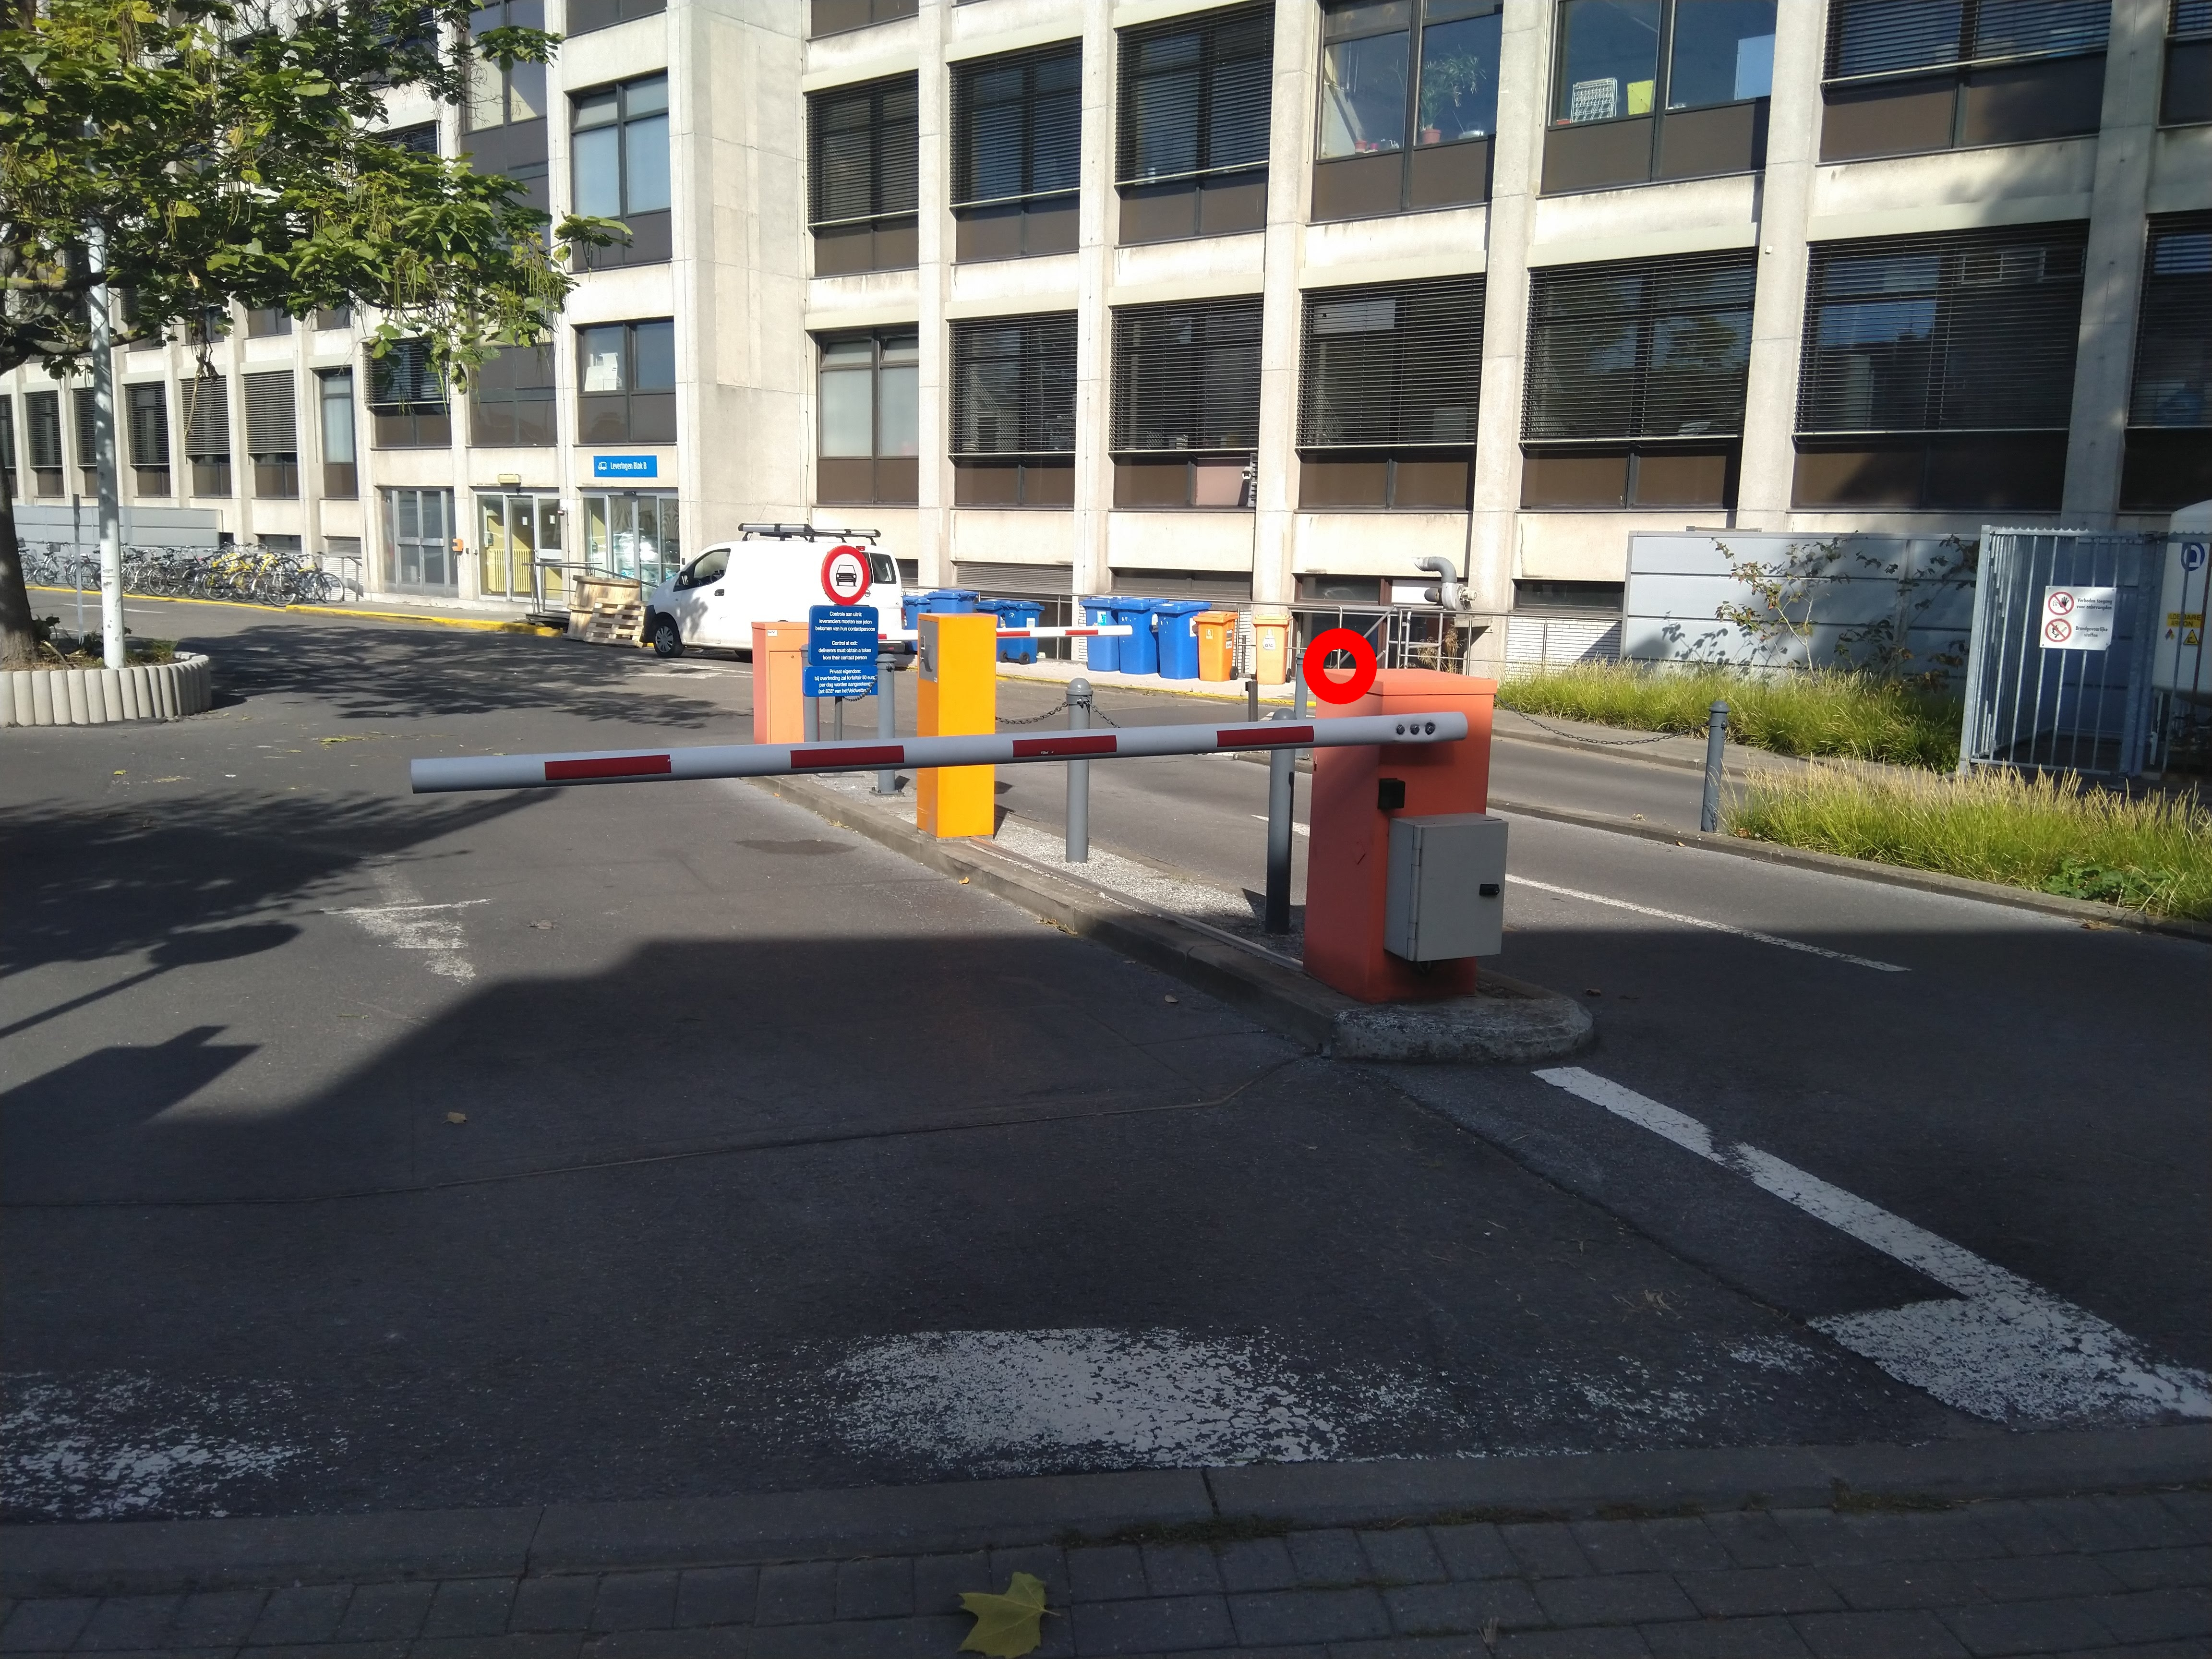
\includegraphics[width=0.4\linewidth]{../bachproef/img/kruisboog/kruisboog-uitgang.jpg}
	\includegraphics[width=0.4\linewidth]{../bachproef/img/res-galglaan/galg.jpg}
	\includegraphics[width=0.4\linewidth]{../bachproef/img/depintelaanorigineel.jpg}
	\includegraphics[width=0.4\linewidth]{../bachproef/img/coupure-links/coupure-links.jpg}
\end{center}

Volgende resultaten zijn bekomen per uitgang. De twee tabellen beschrijven de resultaten van de detectie per foto en per auto. De resultaten per auto zijn bekomen door de individuele foto's samen te voegen, indien één van de foto's correct is wordt het resultaat als correct gezien. De uitgang aan de Coupure Links zijn niet verwerkt door het tekort aan doorrijdende auto's.

\begin{center}
	\centering
	\begin{tabular}{l|l|l|l|l}
		\textbf{Resultaten per individuele foto}	& \textbf{Totaal}	& \textbf{Incorrect} & \textbf{Correct} & \textbf{Ratio} \\ \hline
		Campus Coupure - Uitgang Kruisboogstraat  & 68 & 16 & 52 & 76.5\% \\
		Campus Sterre - Uitgang Galglaan 		  & 62& 13 & 49 & 79.0\%\\
		Campus Sterre - Uitgang De Pintelaan	  & 64& 19 & 45 & 70.3\%\\ \hline
		Totaal 									  & 194& 48 & 146 & 75.3\%
	\end{tabular}
\end{center}

\begin{center}
	\centering
	\begin{tabular}{l|l|l|l|l}
		\textbf{Resultaten per auto}	& \textbf{Totaal}	& \textbf{Incorrect} & \textbf{Correct} & \textbf{Ratio} \\ \hline
		Campus Coupure - Uitgang Kruisboogstraat& 1 & 25  & 26 & 96.2\% \\
		Campus Sterre - Uitgang Galglaan		& 1 & 22  & 23 & 95.7\%\\
		Campus Sterre - Uitgang De Pintelaan	& 2 & 24  & 26 & 92.0\%\\ \hline
		Totaal 									& 4 & 71 & 75 & 94.7\%
	\end{tabular}
\end{center}

%\color{HoGentAccent1} 
%\section*{Sectie met figuur}
%\color{black}


%\begin{center}\vspace{1cm}
%\includegraphics[width=1.0\linewidth]{grail}
%\captionof{figure}{\color{HoGentAccent5} He hasn't got shit all over him. The nose? Where'd you get the coconuts? What do you mean? We shall say 'Ni' again to you, if you do not appease us}
%\end{center}\vspace{1cm}

%------------------------------------------------



\color{HoGentAccent1} 
\section*{Conclusies}
\color{black}
Het doel van dit onderzoek was het nagaan of nummerplaatdetectie een haalbare technologie was aan de UGent Campus Sterre en Campus Coupure. Dit met behulp van een Raspberry Pi met PiCam en de open-source implementatie van OpenALPR die een goedkope oplossing zouden kunnen bieden. Om deze vraag te beantwoorden werd onderzocht of een dergelijke implementatie mogelijk is met de intrede van de GDPR, en of deze wel degelijk goede resultaten kan opleveren op de uitgangen van de campussen zelf.

\paragraph{Is nummerplaatdetectie een haalbare techniek omtrent GDPR?}
Om de eerste vraag te beantwoorden werd een literatuurstudie uitgevoerd over de GDPR zelf, dit hield in hoe deze werkt en hoe deze een ANPR-systeem beïnvloedt. Uit de studie bleek dat de wetgeving een zeer grote invloed heeft op een ANPR-detectie implementatie. Foto's en andere persoonsgegevens zijn verplicht zo min mogelijk verwerkt te worden en dit enkel indien dit gerechtvaardigd is. Verder moet het mogelijk zijn voor een betrokkene om deze op te vragen, te corrigeren of te verwijderen.

Een wettelijke implementatie van een ANPR-systeem is wellicht haalbaar. De wettelijke gronden staan de verwerking van de foto's toe op de grond van het gerechtvaardigde belang zolang deze een duidelijke doelbinding hebben en niet voor andere zaken gebruikt worden. Functionaliteiten zoals het aanpassen van persoonsgegevens of het beveiligen van de gegevens zouden normaal gezien een hoge implementatiekost hebben om hier een systeem rond te bouwen, maar door persoonsgegevens tot een absoluut minimum te houden en de betrokkene niet identificeerbaar te maken is deze functionaliteit niet vereist en dekt men implementatiekosten. Dit maakt het mogelijk om een implementatie goedkoop te maken en aldus haalbaarder.

\paragraph{Welke maatregelen moeten er genomen worden om succesvol nummerplaatdetectie te implementeren?}
Uit de tweede literatuurstudie naar maatregelen rond ANPR kwam naar voor dat nummerplaatdetectie vooral afhankelijk is van de gebruikte camera-instellingen en de OpenALPR configuratie. Zo speelt de locatie van de camera een groot belang tegen de interferentie van de koplampen van voertuigen. Deze studie kan dan ook gebruikt worden als richtlijnen voor een fysieke implementatie.

\paragraph{Kan men nummerplaatdetectie succesvol uitvoeren met een Raspberry Pi op de campus Coupure en Sterre van UGent?}
Op basis van de verkregen richtlijnen werd een opstelling gemaakt. Deze haalde een verwachte nauwkeurigheid van gemiddeld 94.7\%, wat overeenkomt met het onderzoek van , waar men in optimale omstandigheden en gelijkaardige technologieën een nauwkeurigheid van 94.4\% behaalde. Deze resultaten doen vermoeden dat een ANPR-systeem wel degelijk mogelijk is aan de uitgangen van UGent. Deze resultaten stellen de weg open naar breder onderzoek op deze locaties.

Voor de opstelling zelf is een relatief goedkope oplossing gevonden. Op twee van de uitgangen was het mogelijk om de camera simpelweg op de metalen constructie van de hefboom te plaatsen, wat kosten omlaag brengt. Voor de uitgang aan de Campus Sterre De Pintelaan was dit helaas niet mogelijk door de vele inrijrichtingen en de interferentie van het zonlicht. Hierdoor is het essentieel om een verhoging of een paal te plaatsen zodat de camera verhoogd kan worden om een degelijk resultaat te verkrijgen. Dit zal de kosten aan deze uitgang doen stijgen i.v.m. andere uitgangen.


%----------------------------------------------------------------------------------------
%	FORTHCOMING RESEARCH
%----------------------------------------------------------------------------------------
\color{HoGentAccent1} 
\section*{Toekomstig onderzoek}
\color{black}
Deze resultaten zijn behaald onder normale weersomstandigheden in zonlicht en lichte regen. Verder onderzoek is nodig om te bevestigen of een dergelijke opstelling succesvol is 's nachts of in hevige weersomstandigheden. Alsook om de detectie aan de uitgang op de Campus Coupure - Uitgang Coupure Links te bepalen.

%----------------------------------------------------------------------------------------

\end{multicols}
\end{document}